\section{An absolute classic}
\subsection{Puff, the magic dragon}

\begin{marginfigure}
      \checkoddpage \ifoddpage \forcerectofloat \else \forceversofloat \fi
      \centering
              \frame{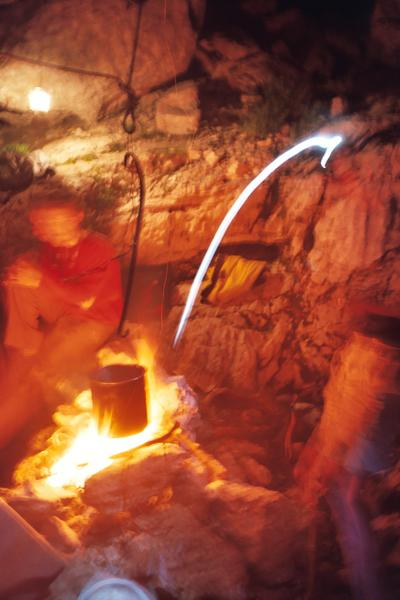
\includegraphics[width=\linewidth]{2007/puff/jarvist frost gr1 film2 -026_23.jpg}} 
  \caption{Making popcorn over the fire. When waiting for the corn to pop or the kettle to boil, singing and otherwise making music is a traditional way to pass the time. \pic{Jarvist Frost}}
\end{marginfigure}

An absolute classic from the \passage{Bivi} on the 2005-07 expos.

\begin{verse}
\begin{centering}
\vspace{3pt}    

\note Puff, the magic dragon lived by the sea 
\newline And frolicked in the autumn mist in a land called honah lee,
\newline Little jackie paper loved that rascal puff,
\newline And brought him strings and sealing wax and other fancy stuff. oh
\par Puff, the magic dragon lived by the sea
\newline And frolicked in the autumn mist in a land called honah lee,
\newline Puff, the magic dragon lived by the sea
\newline And frolicked in the autumn mist in a land called honah lee.
\par Together they would travel on a boat with billowed sail
\newline Jackie kept a lookout perched on puffs gigantic tail,
\newline Noble kings and princes would bow wheneer they came,
\newline Pirate ships would lower their flag when puff roared out his name. oh!
\par Puff, the magic dragon lived by the sea
\newline And frolicked in the autumn mist in a land called honah lee,
\newline Puff, the magic dragon lived by the sea
\newline And frolicked in the autumn mist in a land called honah lee.
\par A dragon lives forever but not so little boys
\newline Painted wings and giant rings make way for other toys.
\newline One grey night it happened, jackie paper came no more
\newline And puff that mighty dragon, he ceased his fearless roar.
\par His head was bent in sorrow, green scales fell like rain,
\newline Puff no longer went to play along the cherry lane.
\newline Without his life-long friend, puff could not be brave,
\newline So puff that mighty dragon sadly slipped into his cave. oh!
\par Puff, the magic dragon lived by the sea
\newline And frolicked in the autumn mist in a land called honah lee,
\newline Puff, the magic dragon lived by the sea
\newline And frolicked in the autumn mist in a land called honah lee. \sidenote {The "Puff" song was originally released by the American folk group \textit{Peter, Paul and Mary} in 1963}

\end{centering}
\end{verse}


\fullwidthbox{Playlists on a 1G SD Card for Mig 2007, along with some Blackadder}{01{\_}jarv{\_}upbeat.pls\\
    02{\_}jarv{\_}mellow.pls\\
    03{\_}bivvi{\_}hits.pls\\
    04{\_}strange.pls\\
    05{\_}love{\_}pop.pls\\
    06{\_}jarv{\_}for{\_}jarv.pls\\
    07{\_}jarv{\_}humour.pls\\
    08{\_}jarv{\_}morvern.pls\\
    09{\_}jarv{\_}for{\_}andy.pls\\
    10{\_}jarv{\_}for{\_}sandeep.pls\\
    11{\_}lock.pls\\
    12{\_}last{\_}mix.pls\\
    13{\_}alt{\_}pop.pls\\
    
Blackadder. Nuff said.}
